\chapter{Preliminary studies on the \texorpdfstring{\lambdadecay}{Lambda baryon decay} angular distribution}
\label{cap:angular_distribution}

@todo: intro

Unless otherwise specified, results and plots in this chapter are obtained with simulated \demonstratorshort events with all selection steps from Chapter \ref{cap:event_selection} applied (prefilters, \bz invariant mass veto, \kshort Armenteros-Podolanski veto and HBDT hard threshold cut) and selecting the $\mu \pm 3\sigma$ signal region, using $\mu$ and $\sigma$ best values from the Run 2 data $J/\psi\,\Lambda^0$ invariant mass fit (see Table \ref{tab:4:fit_results}).

\section{Proton angular distributions}
As described in Section \ref{sec:lambda}, \lz polarization $\vec{s}$ after the magnet can be computed by fitting the proton angular distribution
\begin{equation*}
	\frac{dN}{d\Omega'} = 1+ \alpha \vec{s} \cdot \hat{k}',
	\tag{\ref{eq:angular_distribution_cap1} revisited}
\end{equation*}
with unit vector
\begin{equation*}
\hat{k}'
=
\begin{pmatrix}
	\sin \theta' \cos \phi' \\
	\sin \theta' \sin \phi' \\
	\cos \theta'
\end{pmatrix},
\tag{\ref{eq:1:k_hat} revisited}
\end{equation*}
pointing in the flight direction $\Omega' \coloneqq (\theta',\phi')$ of the proton in the \lz rest frame.
I compute the helicity angle in the \slambda frame, whereby the $z$ axis is defined by the \lz momentum direction $\hat{p}_\Lambda^H$ in the \lbz rest frame \shad (depicted in Figure \ref{fig:1:frames_of_reference_heavy}).
This is the frame where initial \lz polarization is maximal, thus preventing the Wick dilution effect that arises when using the \slambdal frame (see Section \ref{info:wick}).

We define the heavy hadron \lbz rest frame coordinate system $(x_0^H, y_0^H, z_0^H)$, with
\begin{equation}
	\hat{z}_0^H = \hat{p}_{\Lambda_b}^\text{L}
\end{equation}
pointing towards the \lbz momentum in the laboratory frame and $x_0^H, y_0^H$ lying on the \demonstratorshort decay plane.
The \slambda rest frame can be reached from the \lbz rest frame via the rotation operator $R(\phi,\theta,0)$, with $\theta$ and $\phi$ being the \lz helicity angles shown in Figure \ref{fig:1:frames_of_reference_heavy}:
a rotation of angle $\phi$ about the $z_0^H$ axis sends
$(x_0^H, y_0^H, z_0^H) \rightarrow (x_1^H, y_1^H, z_1^H)$ and a $\theta$ rotation about  $y_1^H$ sends $(x_1^H, y_1^H, z_1^H) \rightarrow (x_2^H, y_2^H, z_2^H)$.
The final rotation about $z_2^H$ is not necessary and conventionally set to zero \cite{Richman:153636} \cite{Jurik:2206806}.
This twice-rotated frame defines the \slambda helicity frame coordinate system used to compute $\theta',\phi'$ for \eqref{eq:angular_distribution_cap1}:
\begin{equation}
	\begin{cases}
		\hat{x}_0^\Lambda = \hat{x}_2^H, \\
		\hat{y}_0^\Lambda = \hat{y}_2^H, \\
		\hat{z}_0^\Lambda = \hat{z}_2^H.
	\end{cases}
\end{equation}

In practice, the $z_0^\Lambda$ direction is the easiest to compute, as by definition of \slambda it's the \lbz momentum unit vector in the \shad frame:
\begin{equation}
	\hat{z}_0^\Lambda = \hat{z}_2^H = \vec{p}_\Lambda^H.
\end{equation}
%\begin{equation}
%	\vec{a}_{\Lambda \perp z_0}^H
%	=
%	\left(\vec{p}_\Lambda^H\right)_{\perp z_0^H}
%	=
%	\vec{p}_\Lambda^H - \left(\vec{p}_\Lambda^H\right)_{\parallel z_0^H}
%\end{equation}
%
%\begin{equation}
%	\hat{x}_1^H = \hat{a}^H_{\Lambda \perp z_0}
%\end{equation}
Axis $\hat{x}_0^\Lambda = \hat{x}_2^H$ is defined as the antiparallel unit vector to the component of $\hat{z}_1^H$ that is perpendicular to $\hat{z}_2^H = \vec{p}_\Lambda^H$.
An extensive treatment of the first rotation is superfluous for our end goal:
since said rotation is about $\hat{z}_0^H$, obviously $\hat{z}_1^H = \hat{z}_0^H$ and we can determine $\hat{x}_0^\Lambda$ by computing the $\hat{z}_0^H$ component perpendicular to
%the \lz momentum in \shad frame.
$\vec{p}_\Lambda^H$.
This is done by vector-subtracting its projection on $\vec{p}_\Lambda^H$ from $\hat{z}_0^H$ itself:
\begin{equation}
	\vec{a}^H_{\hat{z}_0 \perp \Lambda}
	\coloneqq
	\left(\hat{z}_0^H\right)_{\perp \vec{p}_\Lambda^H}
	=
	\hat{z}_0^H - \left(\hat{z}_0^H\right)_{\parallel \vec{p}_\Lambda^H},
\end{equation}
\begin{equation}
	\hat{x}_0^\Lambda = \hat{x}_2^H
	=
	- \hat{a}^H_{\hat{z}_0 \perp \Lambda}.
\end{equation}
The $y_0^\Lambda$ axis is fixed by the Cartesian coordinate convention:
\begin{equation}
	\hat{y}_0^\Lambda = \hat{z}_0^\Lambda \times \hat{x}_0^\Lambda
\end{equation}
Within this newfound coordinate system we can compute the proton $\theta$ and $\phi$ helicity angles
\begin{subequations}
	\label{eq:5:helicity_angles}
	\begin{align}
		&\cos\theta_p \coloneqq \cos\theta'
		=
		\hat{z}_0^\Lambda \cdot \hat{p}_p^\Lambda,
		\label{eq:5:helicity_theta} \\
		%%%%%%%%%%%%%%%%%%%%%%%%%%%%%%%
		&\phi_p \coloneqq \phi'
		=
		\arctantwo
		\left(
			\hat{y}_0^\Lambda \cdot \hat{p}_p^\Lambda,
			\hat{x}_0^\Lambda \cdot \hat{p}_p^\Lambda
		\right),
		\label{eq:5:helicity_phi}
	\end{align}
\end{subequations}
with momenta computed in the \lz rest frame via a double Lorentz boost (laboratory frame into \lbz rest frame into \lz rest frame).

\begin{figure}[t]
	\centering
	\begin{subfigure}{.45\textwidth}
		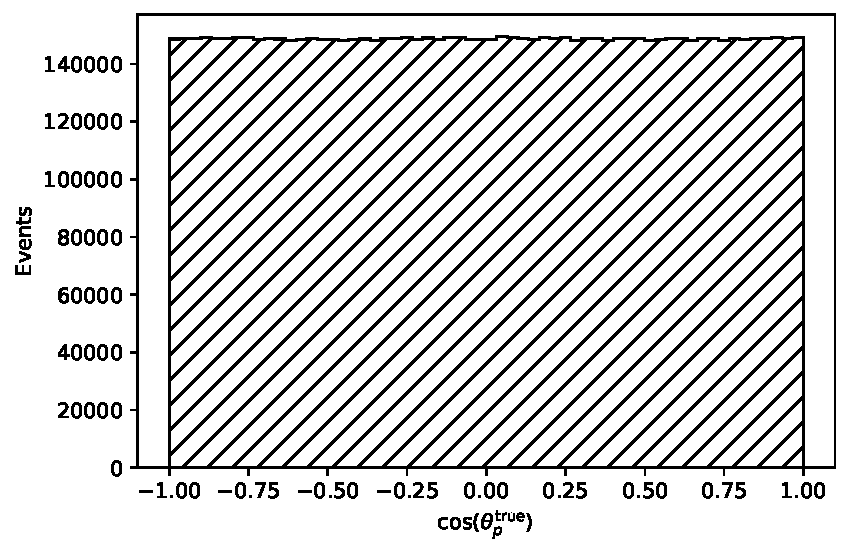
\includegraphics[height=.2\textheight]{graphics/05-angular_distributions/MCTRUTH_theta_true.pdf}
		\caption{}
		\label{fig:5:MCTRUTH_theta_true}
	\end{subfigure}
	\begin{subfigure}{.45\textwidth}
		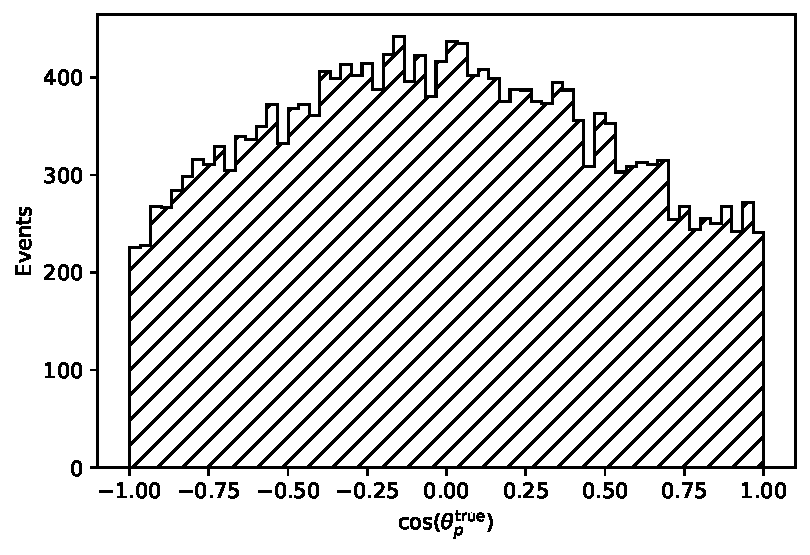
\includegraphics[height=.2\textheight]{graphics/05-angular_distributions/MCRECO_theta_true.pdf}
		\caption{}
		\label{fig:5:MCRECO_theta_true}
	\end{subfigure}
	\caption{Distributions of true values of \cthetap, as defined in \eqref{eq:5:helicity_theta}, for simulated \demonstratorshort events after all selection steps: \textit{(a)} using all generated events; \textit{(b)} using only reconstructed events.}
	\label{fig:5:theta_distributions_true}
\end{figure}

\begin{figure}[t]
	\centering
	\begin{subfigure}{.45\textwidth}
		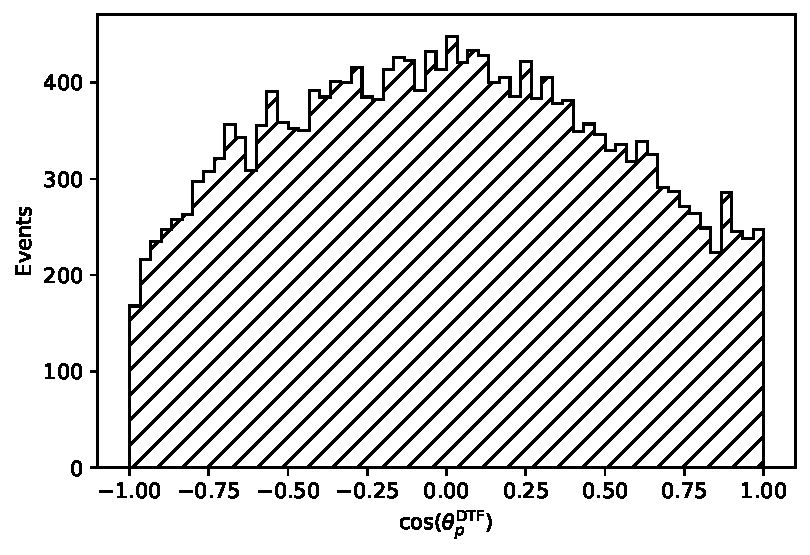
\includegraphics[height=.2\textheight]{graphics/05-angular_distributions/MCRECO_theta_reco.pdf}
		\caption{}
		\label{fig:5:MCRECO_theta_reco}
	\end{subfigure}
	\begin{subfigure}{.45\textwidth}
		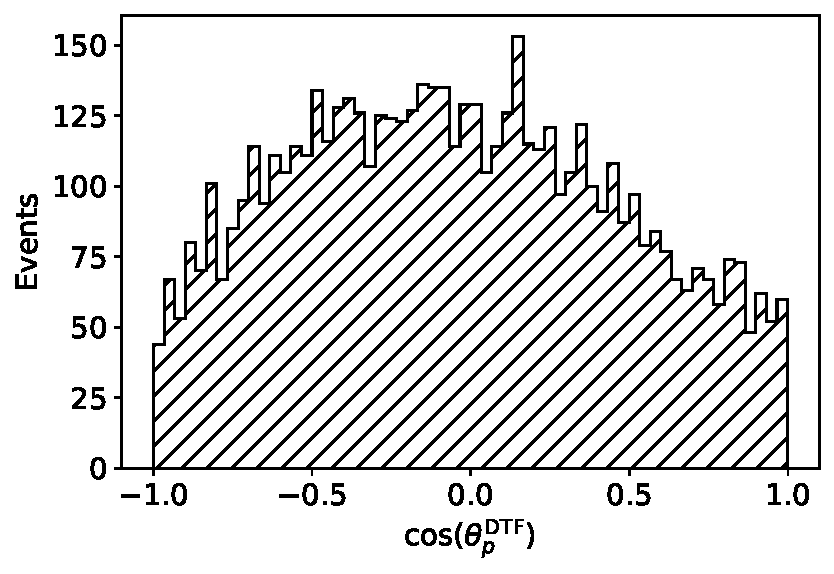
\includegraphics[height=.2\textheight]{graphics/05-angular_distributions/RUN2_theta_reco.pdf}
		\caption{}
		\label{fig:5:RUN2_theta_reco}
	\end{subfigure}
	\caption{Distributions of reconstructed $\cos\theta_p$, as defined in \eqref{eq:5:helicity_theta}, for simulated \demonstratorshort events \textit{(a)} and Run 2 data \textit{(b)} after all selection steps. Angle \thetap is computed using Decay Tree Fitter momenta with \jpsi and \lz mass constraints.}
	\label{fig:5:theta_distributions_reco}
\end{figure}

Figure \ref{fig:5:MCTRUTH_theta_true} depicts the \cthetap distribution of all (including non-reconstructed) simulated \demonstratorshort events using true $p$ and \pim momenta;
these events are generated without accounting for \lz polarization, hence the expected flatness of the distribution.
Figure \ref{fig:5:MCRECO_theta_true} also shows true \cthetap distribution, this time only considering reconstructed events passing all selection steps. The comparison between these two figures highlights the acceptance effects that factor in the prospective \lz EDM/MDM measurement.

Affinity of Figure \ref{fig:5:MCRECO_theta_true} with Figure \ref{fig:5:MCRECO_theta_reco}, which shows reconstructed \cthetap using DTF momenta with \jpsi and \lz mass constraints, foreshadows the great angular resolution I will delve into in Section \ref{sec:5:angular_resolution}.
Finally, \cthetap in Run 2 data after all selection steps is shown in Figure \ref{fig:5:RUN2_theta_reco}:
this distribution is the overlap of contributions from \demonstratorshort signal with polarized \lz and from combinatorial background in the $\mu \pm 3\sigma$ signal region.

%\begin{figure}[t]
%	\centering
%	\begin{subfigure}{.45\textwidth}
%		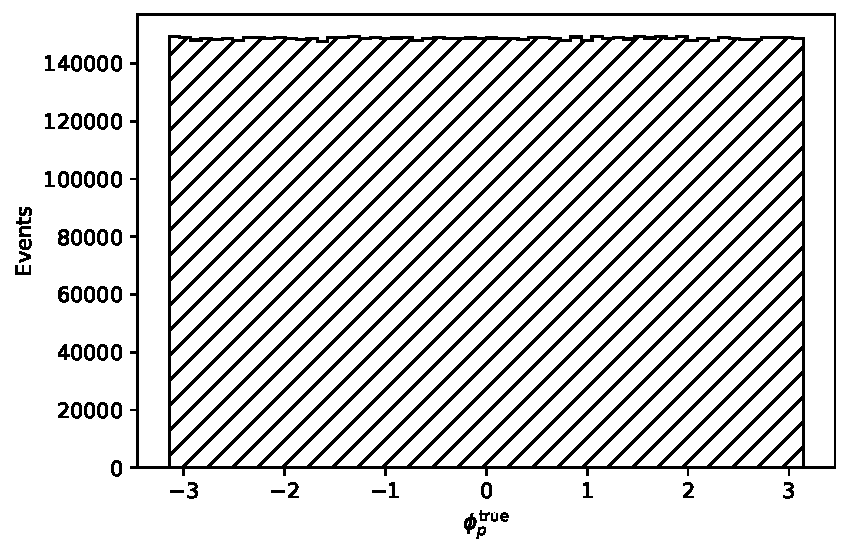
\includegraphics[height=.2\textheight]{graphics/05-angular_distributions/MCTRUTH_phi_true.pdf}
%		\caption{}
%		\label{fig:5:MCTRUTH_phi_true}
%	\end{subfigure}
%	\begin{subfigure}{.45\textwidth}
%		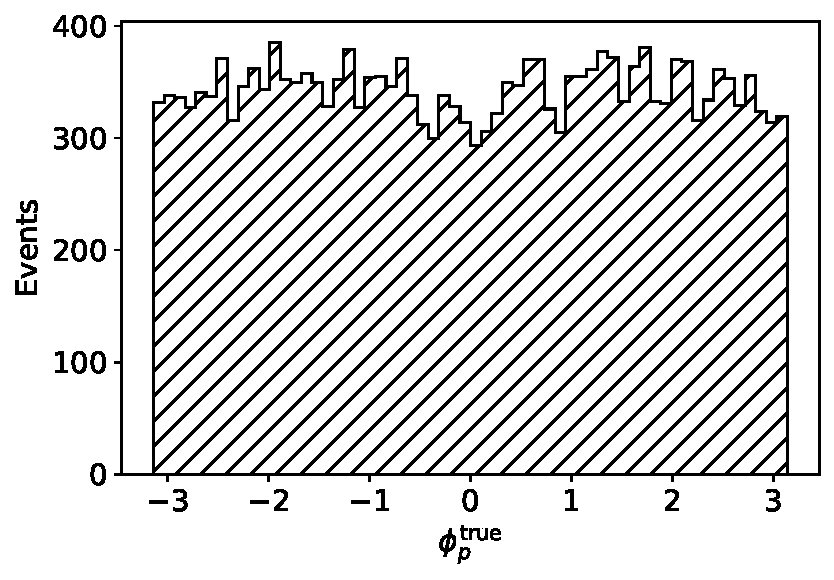
\includegraphics[height=.2\textheight]{graphics/05-angular_distributions/MCRECO_phi_true.pdf}
%		\caption{}
%		\label{fig:5:MCRECO_phi_true}
%	\end{subfigure}
%	\vskip .5\baselineskip
%	\begin{subfigure}{.45\textwidth}
%		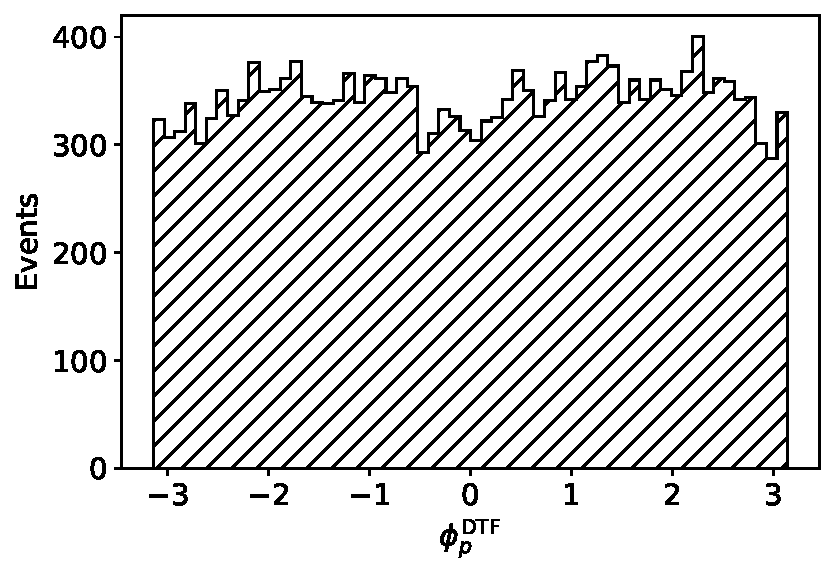
\includegraphics[height=.2\textheight]{graphics/05-angular_distributions/MCRECO_phi_reco.pdf}
%		\caption{}
%		\label{fig:5:MCRECO_phi_reco}
%	\end{subfigure}
%	\caption{Distributions of $\phi_p$, as defined in equation \eqref{eq:5:helicity_phi}, for simulated \demonstratorshort events after all selection steps: \textit{(a)} using all generated events and true momenta; \textit{(b)} using only reconstructed events and true momenta; \textit{(c)} using only reconstructed events and Decay Tree Fitter momenta with \jpsi and \lz mass constraints.}
%	\label{fig:5:phi_distributions}
%\end{figure}

\begin{figure}[t]
	\centering
	\begin{subfigure}{.45\textwidth}
		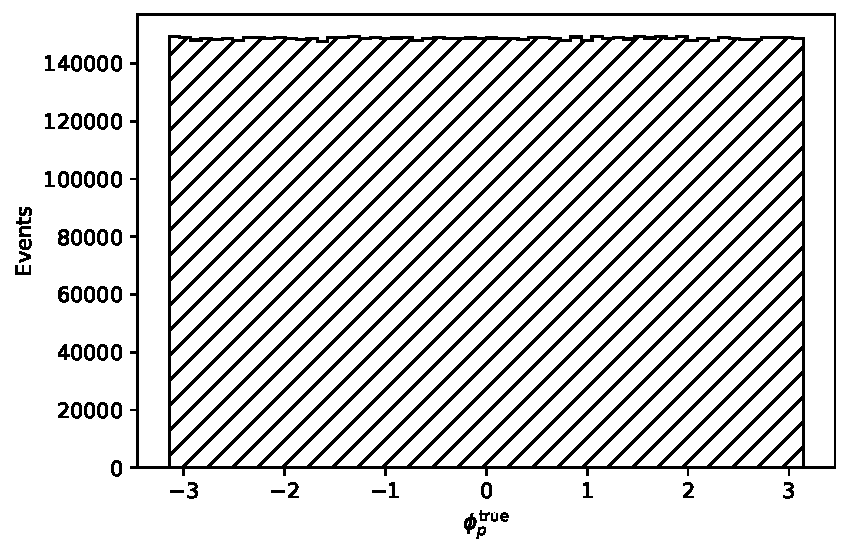
\includegraphics[height=.2\textheight]{graphics/05-angular_distributions/MCTRUTH_phi_true.pdf}
		\caption{}
		\label{fig:5:MCTRUTH_phi_true}
	\end{subfigure}
	\begin{subfigure}{.45\textwidth}
		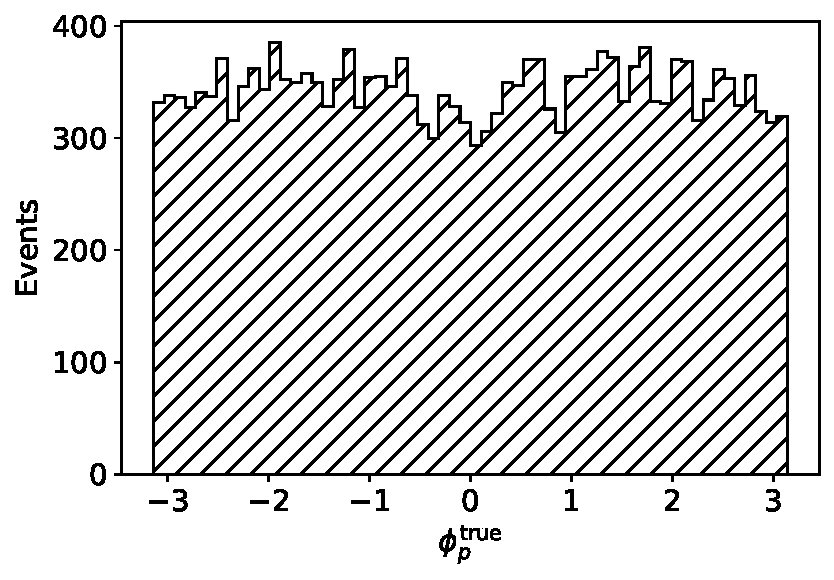
\includegraphics[height=.2\textheight]{graphics/05-angular_distributions/MCRECO_phi_true.pdf}
		\caption{}
		\label{fig:5:MCRECO_phi_true}
	\end{subfigure}
	\caption{Distributions of true values of \phip, as defined in \eqref{eq:5:helicity_phi}, for simulated \demonstratorshort events after all selection steps: \textit{(a)} using all generated events; \textit{(b)} using only reconstructed events.}
	\label{fig:5:phi_distributions_true}
\end{figure}

\begin{figure}[t]
	\centering
	\begin{subfigure}{.45\textwidth}
		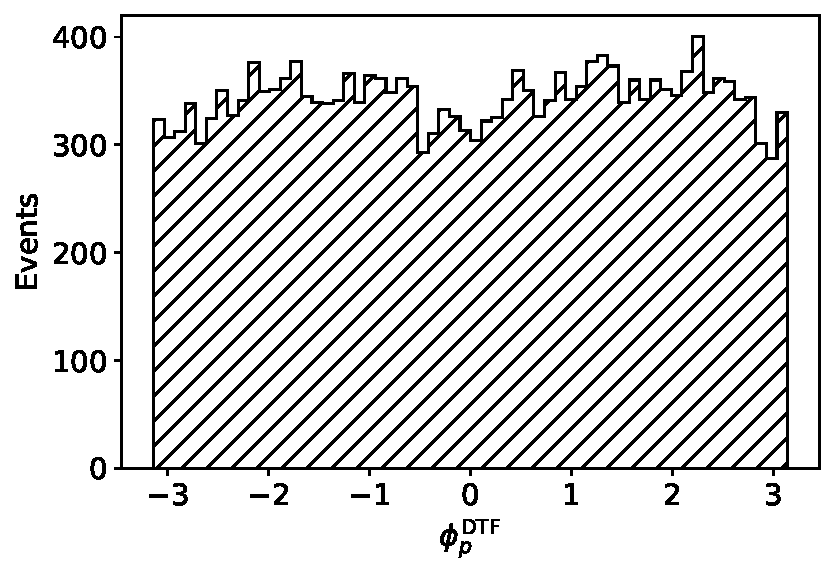
\includegraphics[height=.2\textheight]{graphics/05-angular_distributions/MCRECO_phi_reco.pdf}
		\caption{}
		\label{fig:5:MCRECO_phi_reco}
	\end{subfigure}
	\begin{subfigure}{.45\textwidth}
		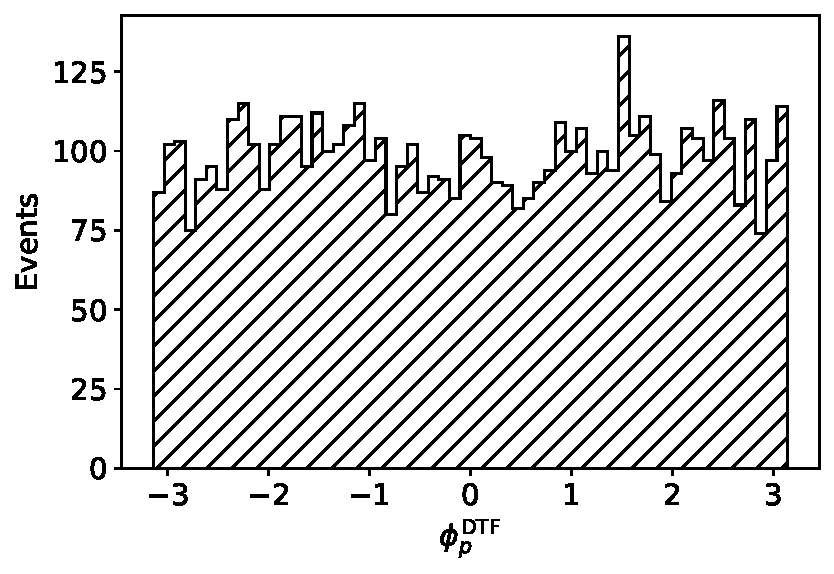
\includegraphics[height=.2\textheight]{graphics/05-angular_distributions/RUN2_phi_reco.pdf}
		\caption{}
		\label{fig:5:RUN2_phi_reco}
	\end{subfigure}
	\caption{Distributions of reconstructed \phip, as defined in \eqref{eq:5:helicity_phi}, for simulated \demonstratorshort events \textit{(a)} and Run 2 data \textit{(b)} after all selection steps. Angle \phip is computed using Decay Tree Fitter momenta with \jpsi and \lz mass constraints.}
	\label{fig:5:phi_distributions_reco}
\end{figure}

The same considerations made for \cthetap are valid for \phip distributions, which are reported in Figures \ref{fig:5:phi_distributions_true} and \ref{fig:5:phi_distributions_reco}.

\section{Proton angular resolution}
\label{sec:5:angular_resolution}

To assess the resolution on the proton angular distribution in reconstructed \demonstratorshort events, I defined 8 $\cos\theta_p^\text{true}$ bins and 12 $\phi_p^\text{true}$ bins and evaluated reconstructed angle dispersion in each truth bin. 
Angular resolution within a bin is defined as the root mean square error (RMSE) between reconstructed and true angles:
\begin{equation}
	\text{RMSE}(\psi) = \sqrt{\frac{1}{N} \sum_{i=1}^N {\left(\psi_i^\text{DTF} - \psi_i^\text{true}\right)}^2},
\end{equation}
with $\psi = \{\cos\theta_p, \phi_p$\}.

\begin{figure}[t]
	\centering
	\begin{subfigure}{.45\textwidth}
		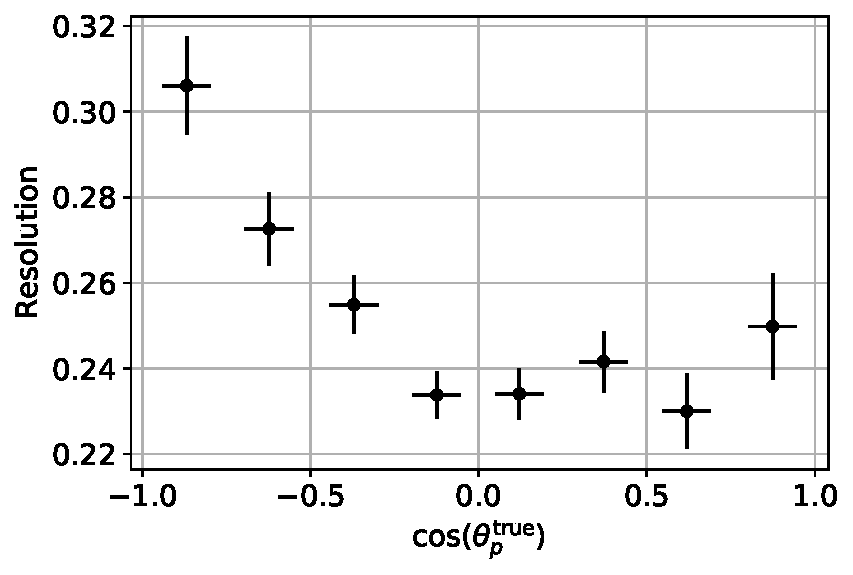
\includegraphics[height=.2\textheight]{graphics/05-angular_distributions/MCRECO_p_theta_resolution.pdf}
		\caption{}
		\label{fig:5:MCRECO_p_theta_resolution}
	\end{subfigure}
	\begin{subfigure}{.45\textwidth}
		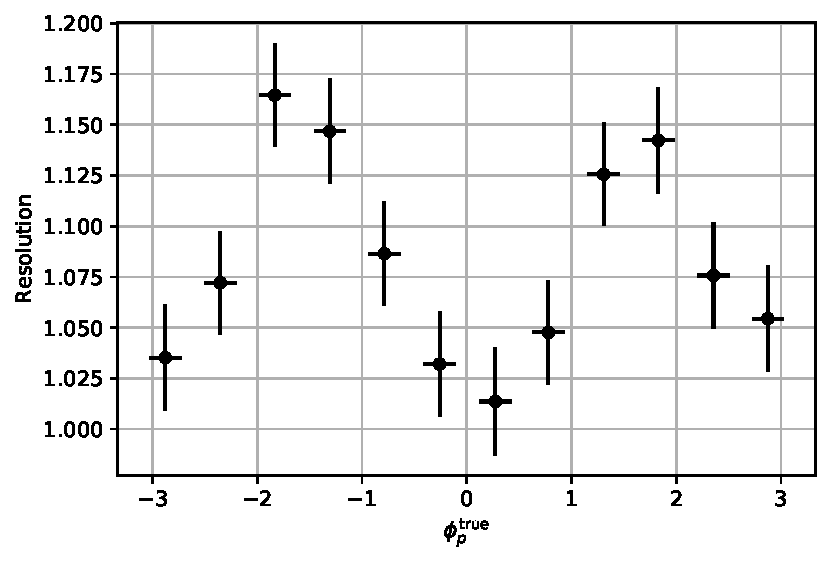
\includegraphics[height=.2\textheight]{graphics/05-angular_distributions/MCRECO_p_phi_resolution.pdf}
		\caption{}
		\label{fig:5:MCRECO_p_phi_resolution}
	\end{subfigure}
	\caption{Resolutions on $\cos\theta_p$ \textit{(a)} and $\phi_p$ \textit{(b)} as a function of the respective true values, computed on simulated \demonstratorshort events after all selection steps.}
	\label{fig:5:angular_resolutions}
\end{figure}

Figure \ref{fig:5:MCRECO_p_theta_resolution} shows \cthetap resolution as a function of $\cos\theta_p^\text{true}$, demonstrating overall good resolution (in line \cthetap variability within each bin).
The asymmetry in resolution at the opposite ends of the \cthetap spectrum, with a marked degradation of resolution around $\cos\theta_p^\text{true} \approx -1$, does not have a clear explanation;
however, as will be seen in Section \ref{sec:5:resolution_after_ghost}, this behaviour becomes a lot less pronounced when the high-bias ghost vertex class of events is removed from the sample.

Figure \ref{fig:5:MCRECO_p_phi_resolution} depicts the same plot for azimuthal helicity angle \phip.
In this case the range of variability for resolution is even smaller, which is consistent with the expected azimuthal symmetry of the LHCb detector;
nevertheless, resolution gets noticeably worse for $\phi_p \approx \pm \frac{\pi}{2}$.
It bears mentioning that the shape of Figure \ref{fig:5:MCRECO_p_phi_resolution} shows remarkable correlation with the observed angular \phip acceptance in reconstructed events (see Figure \ref{fig:5:MCRECO_phi_reco}), suggesting that the two effects might share a common source.

\begin{figure}[t]
	\centering
	\begin{subfigure}{.45\textwidth}
		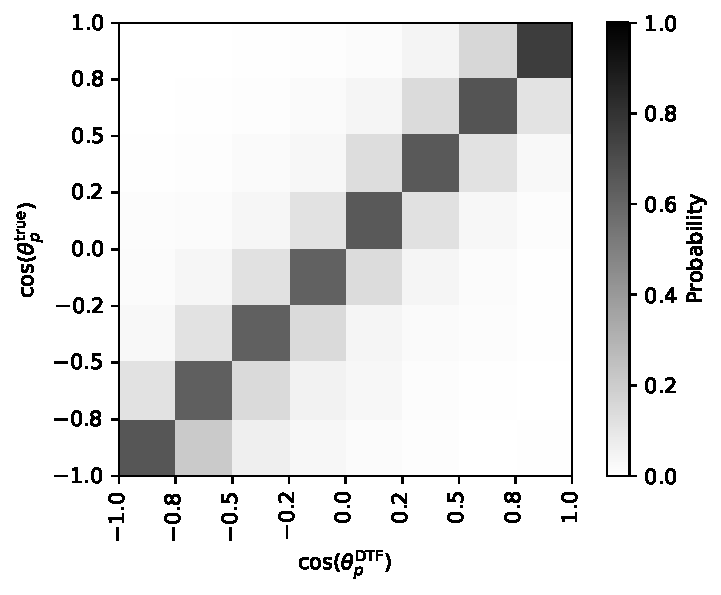
\includegraphics[width=\textwidth]{graphics/05-angular_distributions/MCRECO_p_theta_migration.pdf}
		\caption{}
		\label{fig:5:MCRECO_p_theta_migration}
	\end{subfigure}
	\begin{subfigure}{.45\textwidth}
		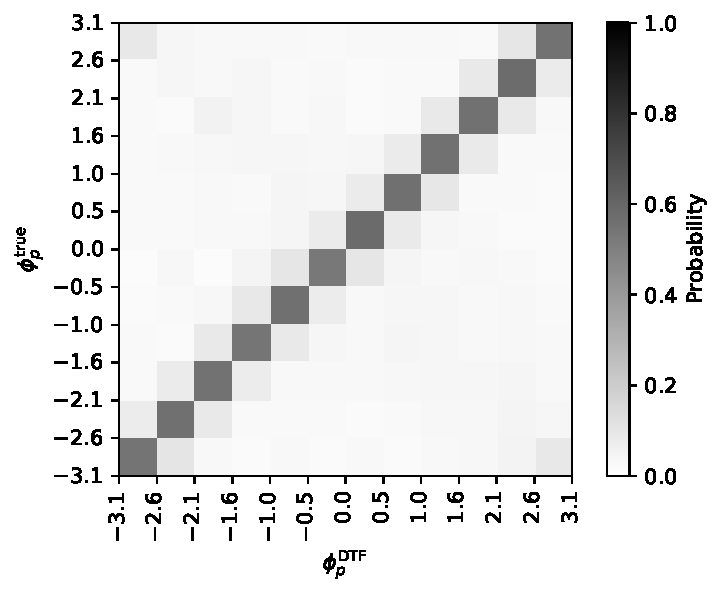
\includegraphics[width=\textwidth]{graphics/05-angular_distributions/MCRECO_p_phi_migration.pdf}
		\caption{}
		\label{fig:5:MCRECO_p_phi_migration}
	\end{subfigure}
	\caption{Migration matrices of $\cos\theta_p$ \textit{(a)} and $\phi_p$ \textit{(b)}, computed on simulated \demonstratorshort events after all selection steps. Probabilities and chromatic scale are normalized on true bins.}
	\label{fig:5:angular_migration_matrices}
\end{figure}

\subsection{\texorpdfstring{\lz}{Lambda} decay vertex bias and ghost vertex events}
\label{sec:lambda_endvertex_bias}

The quality of the \lambdadecay vertex reconstruction affects many aspects of the $\Lambda^0$ electromagnetic dipole moments measurement:
on top of being fundamental to evaluate how much magnetic field the particle traversed (and thus the extent of spin precession), even the best momentum resolution for protons and pions is worthless if the particles are extrapolated at the wrong point of production.
Both $x_\text{vtx}^\Lambda$ and $y_\text{vtx}^\Lambda$ are fairly well reconstructed, with resolution $\lesssim \SI{1}{\centi\meter}$ and no discernible bias.
This section will therefore focus on the reconstruction of $z_\text{vtx}^\Lambda$.

%\begin{figure}[t]
%	\centering
%	\begin{subfigure}{.45\textwidth}
%		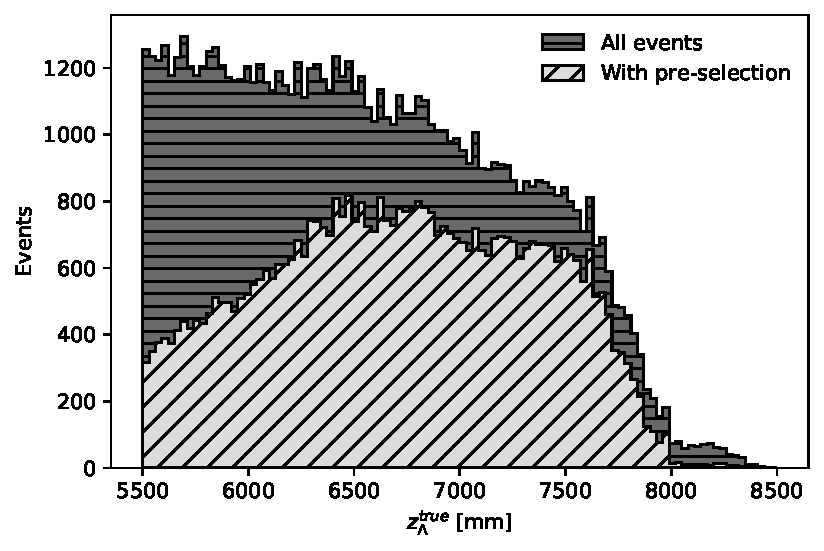
\includegraphics[height=.2\textheight]{graphics/04-event_selection/Lambda_endvertex_z_true.pdf}
%		\caption{}
%		\label{fig:4:lz_vertex_true}
%	\end{subfigure}
%	\begin{subfigure}{.45\textwidth}
%		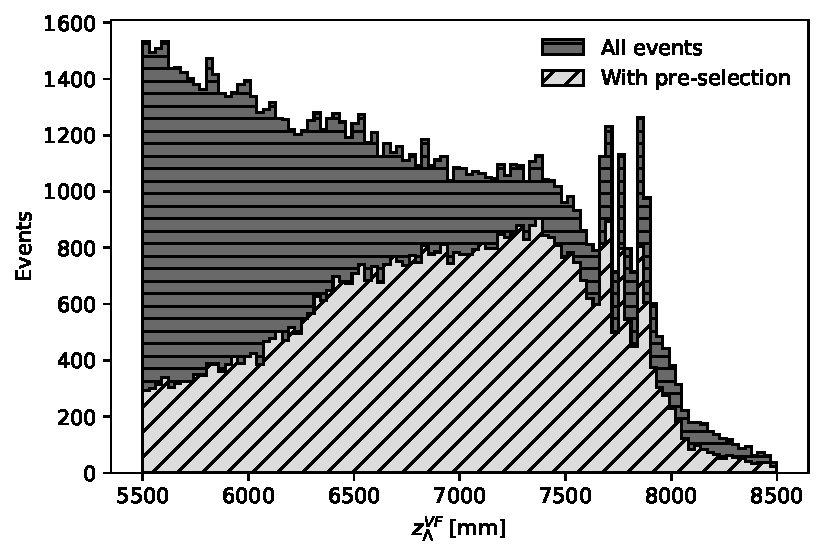
\includegraphics[height=.2\textheight]{graphics/04-event_selection/Lambda_endvertex_z.pdf}
%		\caption{}
%		\label{fig:4:lz_vertex_reco}
%	\end{subfigure}
%	\caption{Distribution of true \textit{(a)} and reconstructed \textit{(b)} $z_\text{vtx}^\Lambda$ in simulated \demonstratorshort signal events, without (\textit{dark grey}) and with (\textit{light grey}) prefiltering.}
%	\label{fig:4:lz_vertex_distributions}
%\end{figure}
%
%\begin{figure}[t]
%	\centering
%	\begin{subfigure}{.45\textwidth}
%		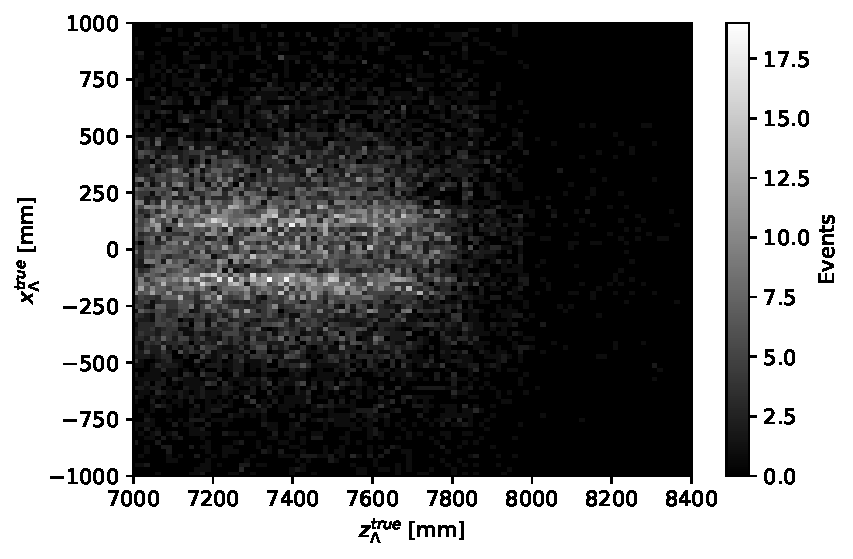
\includegraphics[height=.2\textheight]{graphics/04-event_selection/Lambda_endvertex_z_vs_x_true.pdf}
%		\caption{}
%		\label{fig:4:lz_vertex_peaks_true}
%	\end{subfigure}
%	\begin{subfigure}{.45\textwidth}
%		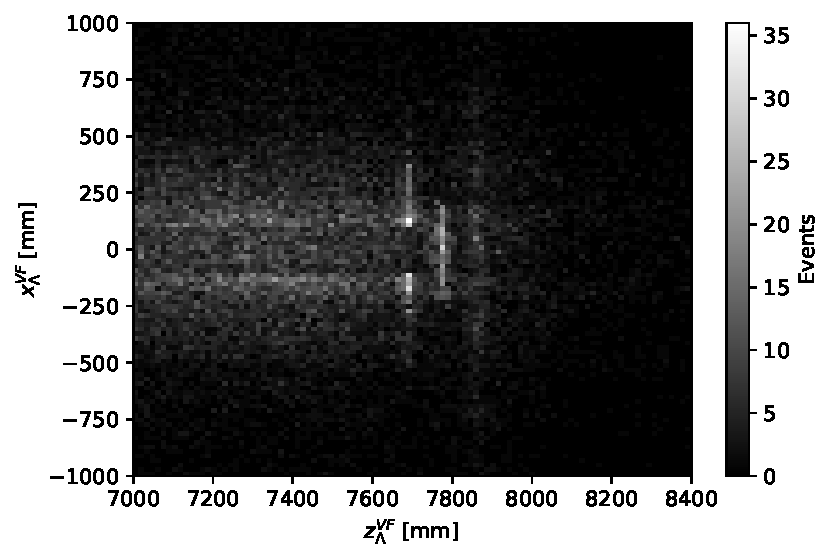
\includegraphics[height=.2\textheight]{graphics/04-event_selection/Lambda_endvertex_z_vs_x.pdf}
%		\caption{}
%		\label{fig:4:lz_vertex_peaks_reco}
%	\end{subfigure}
%	\caption{Distribution of simulated \demonstratorshort signal events (prefilters applied) with $z_\Lambda^\text{VF} \geq \SI{7.0}{\meter}$, as function of true (\textit{left}) and reconstructed (\textit{right}) $x_\Lambda^\text{vtx}$ and $z_\text{vtx}^\Lambda$. This corresponds to a top view of true and reconstructed \lz decay vertices.}
%	\label{fig:4:lz_vertex_peaks}
%\end{figure}
%
%Figures \ref{fig:4:lz_vertex_true} and \ref{fig:4:lz_vertex_reco} show the distributions of true and reconstructed $z_\text{vtx}^\Lambda$ respectively for simulated signal events.
%The most prominent difference between the two is the presence of three peaks in the $[\SI{7.5}{\meter},\SI{8.0}{\meter}]$ region of the reconstructed distribution, being found both with and without prefilter selections. 
%The significance of these structures can be inferred by plotting the events as function of  $z_\text{vtx}^\Lambda$ and $x_\text{vtx}^\Lambda$, corresponding to a bending plane perspective of the detector.
%This is shown in Figure \ref{fig:4:lz_vertex_peaks_reco}, highlighting the fact that the peaks in $\Lambda^0$ decay vertices have a very precise geometrical location, absent when comparing the true $z_\text{vtx}^\Lambda$ and $x_\text{vtx}^\Lambda$ values for the same events (Figure \ref{fig:4:lz_vertex_peaks_true}).
%The spatial distribution of the vertices bears a striking resemblance to the layout of a T tracking station (see Figure \ref{fig:2:t_station_top}) and $z$ coordinates are consistent with the nominal placement of IT and first OT plane of the T1 station \cite{Barbosa-Marinho:582793}.
%While dedicated studies are required to gain more insight into the source of these structures, they are assumed to be of minor impact for the purposes of this thesis.

%The differing shapes of true and reconstructed $z_\text{vtx}^\Lambda$ distributions from Figure  are also evidence of bias effects in the \lambdadecay vertex reconstruction.

\begin{figure}[t]
	\centering
	\begin{subfigure}{.45\textwidth}
		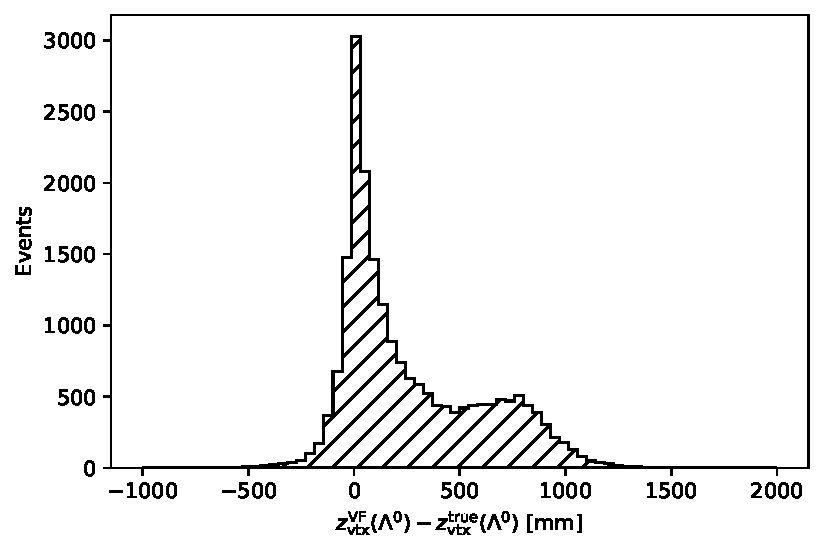
\includegraphics[width=\textwidth]{graphics/05-angular_distributions/Lambda_endvertex_bias_z.pdf}
		\caption{}
		\label{fig:5:lz_endvertex_bias_linear}
	\end{subfigure}
	\begin{subfigure}{.45\textwidth}
		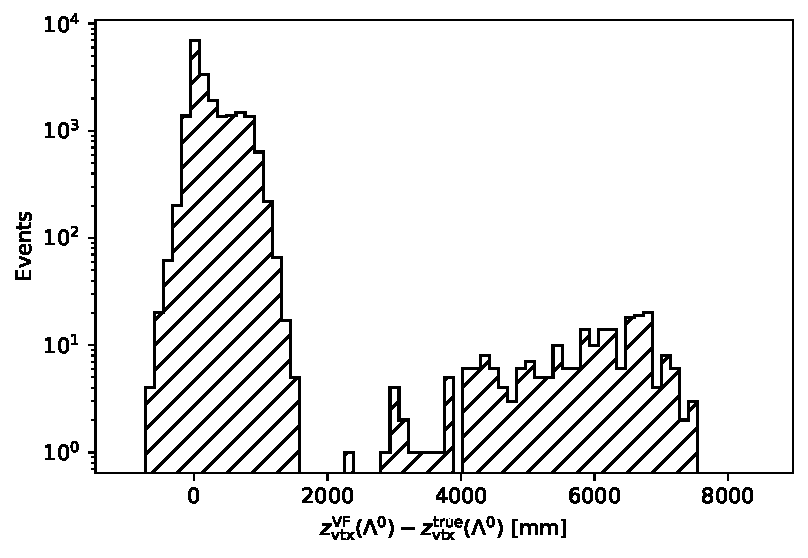
\includegraphics[width=\textwidth]{graphics/05-angular_distributions/Lambda_endvertex_bias_z_log.pdf}
		\caption{}
		\label{fig:5:lz_endvertex_bias_log}
	\end{subfigure}
	\caption{Distribution of $z_\text{vtx}^\Lambda$ bias in linear \textit{(a)} and logarithmic \textit{(b)} scales for simulated \demonstratorshort events after all selection steps.}
	\label{fig:5:lz_endvertex_bias}
\end{figure}

The distribution of $z_\text{vtx}^\Lambda$ residuals for simulated signal events is shown in Figure \ref{fig:5:lz_endvertex_bias_linear}.
Its shape is distinctly non-gaussian, with a second core towards the positive end of the axis counterbalancing the expected $\approx 0$ peak, confirming the presence of a median bias of $\approx \SI{14}{\centi\meter}$\footnote{This number is of course much lower than the $\approx \SI{40}{\centi\meter}$ median bias of Vertex-Fitter-converging events mentioned in Chapter \ref{cap:vertex_reconstruction}. Here not only am I directly selecting $z_\text{vtx}^\Lambda > \SI{5}{\meter}$, which reduces the extent of possible vertex bias given the position of the T stations around \SI{8}{\meter}, but many selection steps are also in place to skim out most badly reconstructed events.}.

\begin{figure}[t]
	\centering
	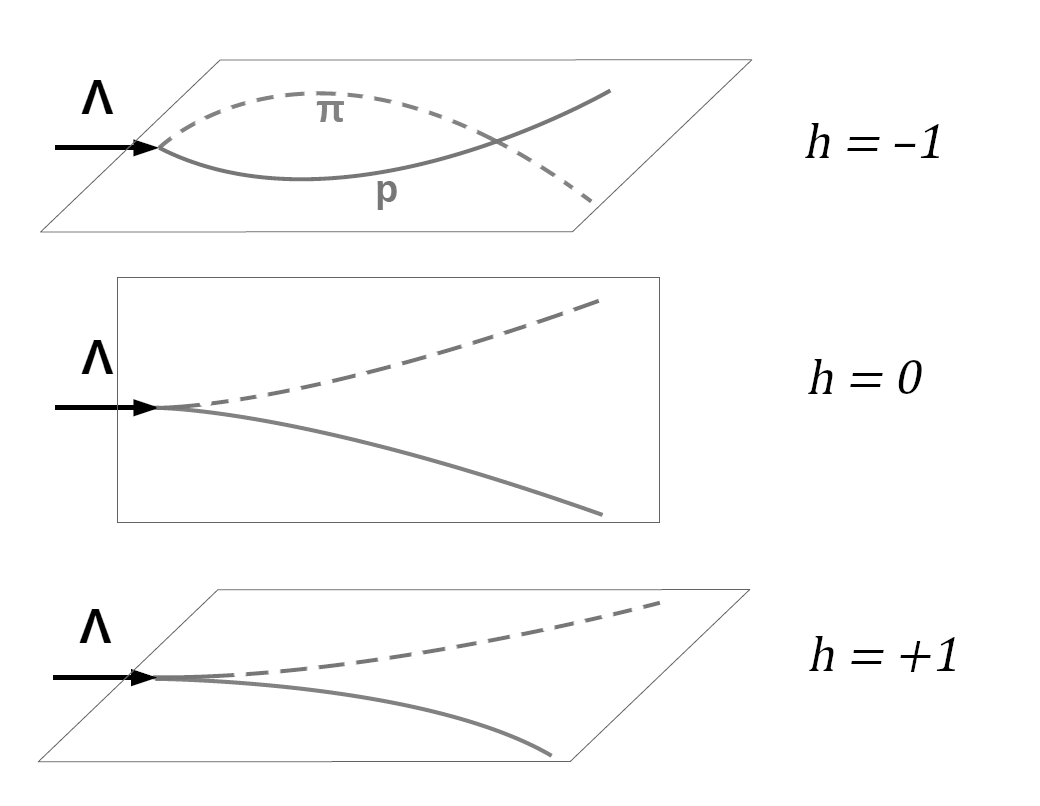
\includegraphics[width=.7\textwidth]{graphics/04-event_selection/horizontality_illustration_bw.png}
	\caption{Depiction of three \lambdadecay configurations and the associated horizontality values. The horizontal planes in the top and bottom diagrams are aligned to the LHCb $xz$ plane, the vertical plane in the middle diagram to the $yz$ plane.}
	\label{fig:4:horizontality_explanation}
\end{figure}

The positive bias core can be interpreted as a mistake the vertexing algorithm commits when confronted with a specific decay geometry.
When the \lambdadecay decay plane closely aligns with the $xz$ bending plane, the bending induced by the magnet can produce either \textit{opening} or \textit{closing} tracks (depicted in top and bottom diagrams respectively in Figure \ref{fig:4:horizontality_explanation}.
In the latter case the tracks will cross again at $z>z_\text{vtx}^\Lambda$;
if $y$ displacement is sufficiently small, the algorithms may converge on this <<ghost>> vertex instead of the real one.

\begin{figure}[t]
	\centering
	\begin{subfigure}{.45\textwidth}
		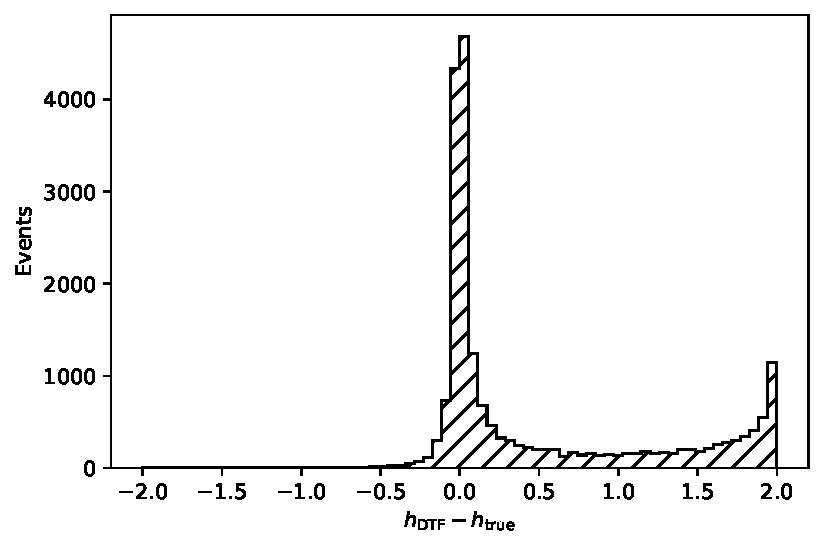
\includegraphics[width=\textwidth]{graphics/05-angular_distributions/Lambda_horizontality_bias.pdf}
		\caption{}
		\label{fig:5:horizontality_bias}
	\end{subfigure}
	\begin{subfigure}{.45\textwidth}
		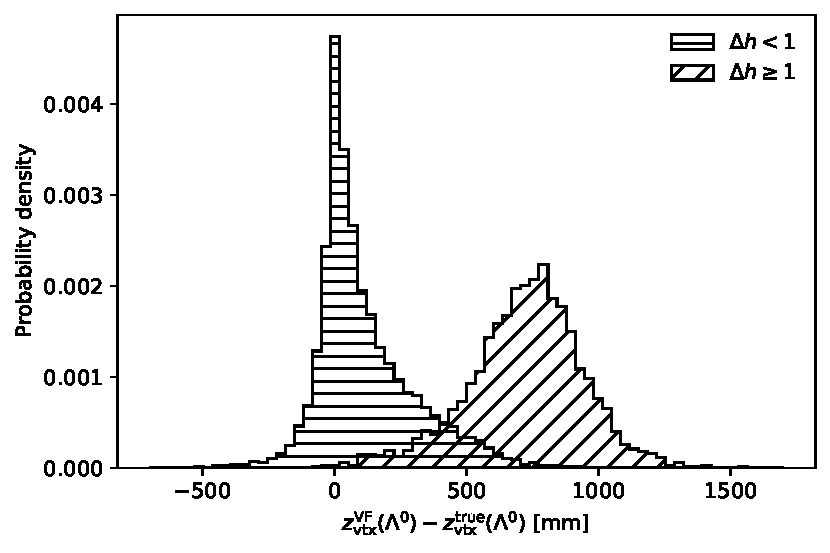
\includegraphics[width=\textwidth]{graphics/05-angular_distributions/lambda_endvertex_z_bias_vs_horizontality_bias.pdf}
		\caption{}
		\label{fig:5:lz_endvertex_bias_vs_horizontality_bias}
	\end{subfigure}
	\caption{\textit{(a)} Bias in horizontality (as defined in \eqref{eq:4:horizontality}) of \lambdadecay decays from simulated \demonstratorshort events. Bias is obtained as the difference between $h_\text{DTF}$ (computed with Decay Tree Fitter momenta with \jpsi and \lz mass constraints) and $h_\text{true}$ (computed with true momenta). \textit{(b)} Distribution of $z_\text{vtx}^\Lambda$ bias for events with horizontality bias $<1$ (\textit{horizontal hatching}) and $\geq 1$ (\textit{diagonal hatching}).}
\end{figure}

To test out this hypothesis we define the \textit{horizontality} of a \lambdadecay event as follows:
\begin{equation}
h = \sign{\left(\Lambda^0_\text{PID}\right)} \sign{\left(B_y\right)}~\frac{a_y}{\lvert \vec{a} \rvert},
\label{eq:4:horizontality}
\end{equation}
where
\begin{equation}
\vec{a} \coloneqq \vec{p}_p \times \vec{p}_\pi 
\end{equation}
is the cross product of proton and pion momenta at production vertex, $\sign{\left(B_y\right)}$ is the dipole magnet polarity\footnote{The LHCb dipole magnet polarity is reversed roughly twice per month to allow for studies on decay asymmetries \cite{Vesterinen:1642153}. The $B_y > 0$ configuration is conventionally known as \textit{magnet up} polarity, $B_y < 0$ as \textit{magnet down}.}
and $\sign{\left(\Lambda^0_\text{PID}\right)}$ is the sign of the PDG Monte Carlo particle numbering scheme of the mother particle ($+1$ for $\Lambda^0$, $-1$ for $\bar{\Lambda}^0$) \cite{PDG}.

Decays with $h=\pm1$ lie exactly on the $xz$ bending plane, $h=-1$ events having closing $p\pi^-$/$\bar{p}\pi^+$ tracks and $h=+1$ events having opening tracks, while $h=0$ events lie on the $yz$ plane (see Figure \ref{fig:4:horizontality_explanation}).
A sufficiently small $y$ track distance is required for the Vertex Fitter to equivocate the ghost vertex for the real one, otherwise the event will not converge in the $yz$ plane.
It follows that the signature for a ghost vertex event is a difference of $\approx 2$ between the reconstructed horizontality $h_\text{DTF}$ (using DTF momenta with \jpsi and \lz mass constraints) and true horizontality $h_\text{true}$, i.e. $h=-1 \rightarrow +1$.
%A horizontality bias $\Delta h \coloneqq h_\text{reco} - h_\text{true} > 1$ thus becomes the signature of a ghost vertex \lambdadecay event.

Figure \ref{fig:5:horizontality_bias} shows the $\Delta h \coloneqq  h_\text{DTF} - h_\text{true } > 1$ distribution for signal \lambdadecay events, highlighting a strong asymmetry between a large number of $\Delta h \approx 2$ events (closing to opening) and almost no $\Delta h \approx -2$ event (opening to closing).
To isolate ghost vertex events I opted for a conservative $\Delta h > 1$ cut;
this leaves out some events with double crossing in the $xz$ plane, such as those with $h_\text{true} = 0-\varepsilon_1 \rightarrow h_\text{DTF} = 0+\varepsilon_2$, but it's functional for a first look at the effect of ghost vertex reconstruction.

%As per Figure , this issue affects $\approx 25\%$ of reconstructed \demonstratorshort events, most of those being $\Delta h \approx 2$ events (from $h=-1$ to $h=+1$), with almost no event with $\Delta h < -1$.

The \lz decay vertex residual distributions shown in Figure \ref{fig:5:lz_endvertex_bias_vs_horizontality_bias} confirm that ghost vertex events are largely responsible for the high-bias core observed in Figure \ref{fig:5:lz_endvertex_bias_linear}.
Some asymmetry effects are still visible in the $\Delta h < 1$ distribution, with a leftover median bias of $\approx \SI{6.4}{\centi\meter}$.
This suggests that further distorsion effects may be in place either in track reconstruction or in the fitting process and further investigation is warranted.

%%Isolating $\Delta h \geq 1$ events and studying their $z_\text{vtx}^\Lambda$ bias distributions (), it becomes clear that they 
%Significant asymmetry effects are , which is still skewed towards positive bias.
%While not ideal, this is somewhat expected given that the Vertex Fitter algorithm scans for candidate vertices starting from the first measurement position (i.e. the T1--T3 stations) and moving upstream.

\begin{figure}[t]
	\centering
	\begin{subfigure}{.45\textwidth}
		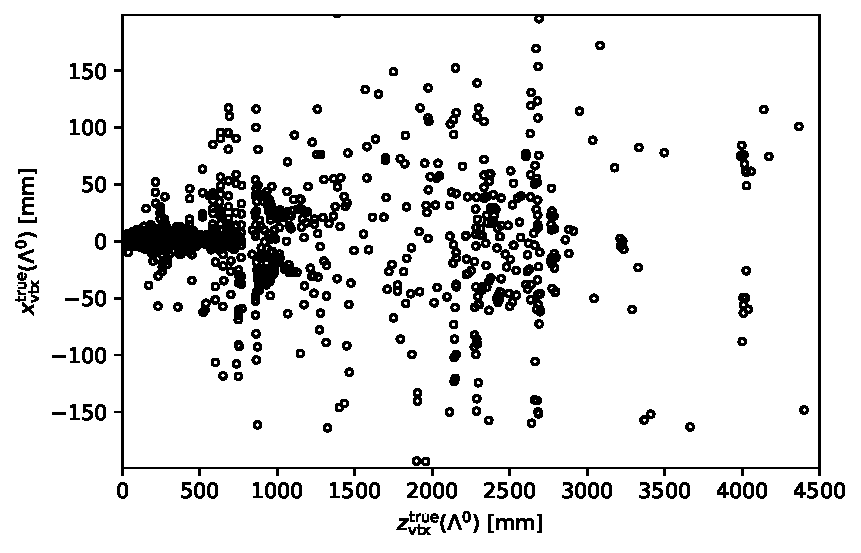
\includegraphics[width=\textwidth]{graphics/05-angular_distributions/bump_Lambda_true_endvertex_z_vs_x.pdf}
		\caption{}
		\label{fig:5:bump_true}
	\end{subfigure}
	\begin{subfigure}{.45\textwidth}
		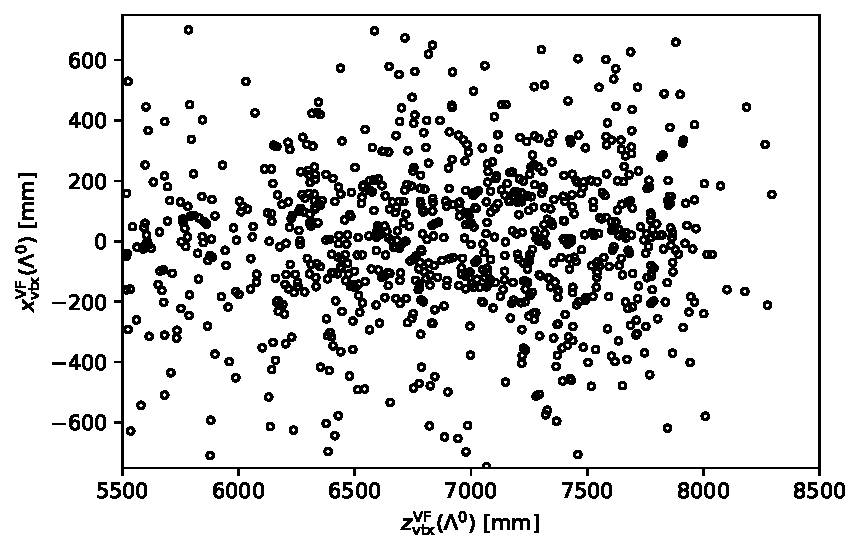
\includegraphics[width=\textwidth]{graphics/05-angular_distributions/bump_scatter_Lambda_endvertex_z_vs_x.pdf}
		\caption{}
		\label{fig:5:bump_reco}
	\end{subfigure}
	\caption{Distribution of simulated \demonstratorshort events (only prefilters applied) with $z_\Lambda^\text{VF} - z_\Lambda^\text{true} \geq \SI{2.0}{\meter}$ as function of true \textit{(a)} and reconstructed \textit{(b)} $x^\Lambda_\text{vtx}$ and $z_\text{vtx}^\Lambda$. This corresponds to a top view of true and reconstructed \lz decay vertices.}
	\label{fig:5:bump}
\end{figure}

Most \demonstratorshort events, even those with ghost vertex reconstruction, still maintain a limited $\lesssim \SI{1.0}{\meter}$ bias on $z_\text{vtx}^\Lambda$.
A smaller substructure with $\geq \SI{2.0}{\meter}$ bias (median bias $\approx \SI{6.0}{\meter}$) emerges when plotting the distribution in logarithmic scale, as seen in Figure \ref{fig:5:lz_endvertex_bias_log}.
These events only amount to $\approx 0.5\%$ of the sample after the selection process, with the fraction raising to $\approx 1.7\%$ when only applying prefilters;
most of them are thus already rejected by the other selection steps.

Figure \ref{fig:5:bump_true} provides a top view of the $\Lambda^0$ decay vertices for this class of events, showing the distribution of true $z_\text{vtx}^\Lambda$ and $x_\text{vtx}^\Lambda$;
to maximize statistics, only prefilters are used.
Most $\Lambda^0$ in high bias events decay in the earlier sections of the detector ($z<\SI{3.0}{\meter}$);
the high spatial concentration in specific regions of the $xz$ plane, such as the <<wings>> around $z\approx \SI{1.0}{\meter}$, as well as the consistency between the placement of these structures and the location of the different LHCb subdetectors (cf. Figure \ref{fig:2:lhcb_diagram}), suggest that they may be the result of interaction with the material.

No dedicated veto on reconstructed variables is possible to filter this class of events:
Figure \ref{fig:5:bump_reco} shows that the $\Lambda^0$ vertices are reconstructed in seemingly arbitrary positions.
Their impact on the overall performance on signal is nevertheless neglectable.

\subsection{Impact of ghost vertex events on proton angular resolution}
\label{sec:5:resolution_after_ghost}

Resolutions reported in Figure \ref{fig:5:angular_resolutions} are computed on a simulated sample with subpar resolution on the \lz decay vertex, as seen from Figure \ref{fig:5:lz_endvertex_bias_linear}.
Roughly $\approx 26\%$ of the data pass the $\Delta h > 1$ criterium, which I have shown to be a good indicator of the fraction of ghost vertex events.
Ongoing studies conducted by the Milan and Valencia LHCb research groups suggest that ghost vertex convergence in double-crossing tracks can be prevented by tweaking the initial vertex seed, which acts as the starting point for the Vertex Fitter algorithm.


\begin{figure}[t]
	\centering
	\begin{subfigure}{.45\textwidth}
		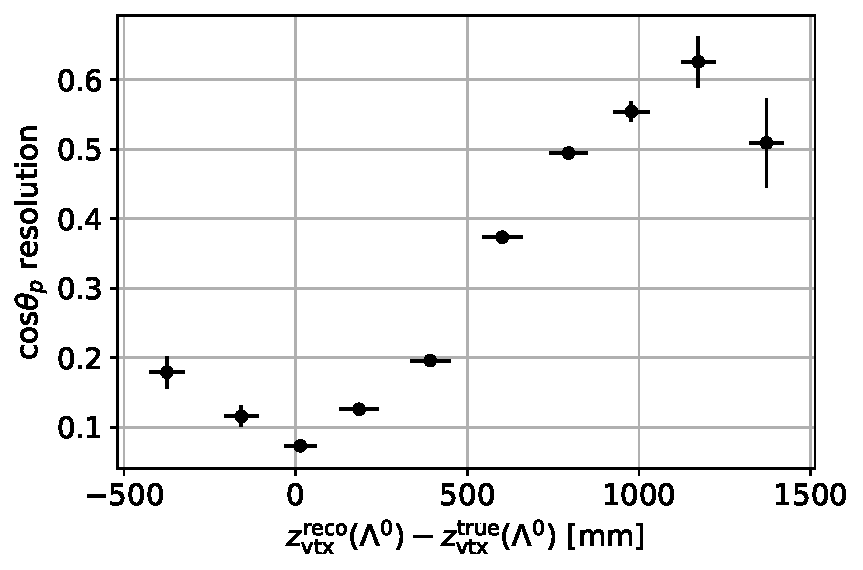
\includegraphics[width=\textwidth]{graphics/05-angular_distributions/MCRECO_p_theta_resolution_vs_L_endvertex_z_bias.pdf}
		\caption{}
		\label{fig:5:theta_resolution_vs_vertex_bias}
	\end{subfigure}
	\begin{subfigure}{.45\textwidth}
		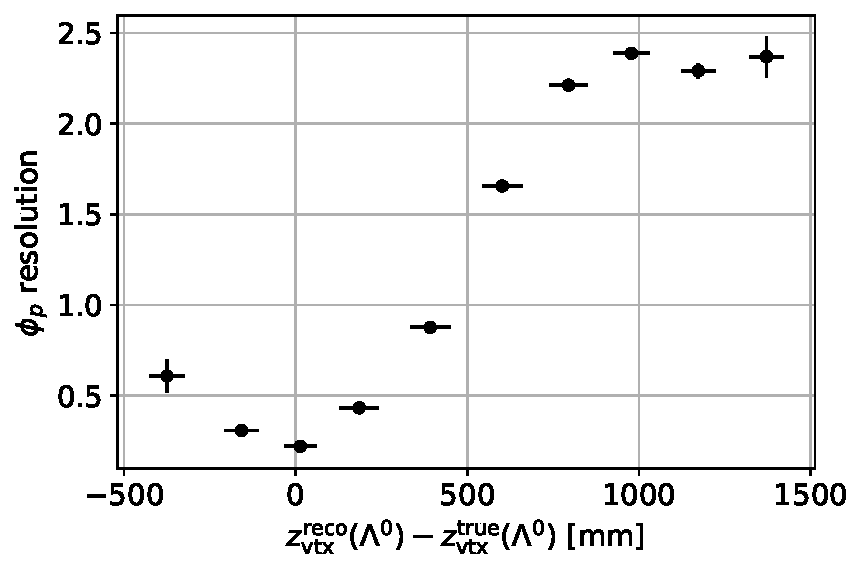
\includegraphics[width=\textwidth]{graphics/05-angular_distributions/MCRECO_p_phi_resolution_vs_L_endvertex_z_bias.pdf}
		\caption{}
		\label{fig:5:phi_resolution_vs_vertex_bias}
	\end{subfigure}
	\caption{Angular resolutions on $\cos\theta_p$ \textit{(a)} and $\phi_p$ \textit{(b)} as a function of bias on reconstructed $z_\text{vtx}^\Lambda$, computed on simulated \demonstratorshort events after all selection steps.}
	\label{fig:5:angular_resolution_vs_vertex_bias}
\end{figure}

\begin{figure}[t]
	\centering
	\begin{subfigure}{.45\textwidth}
		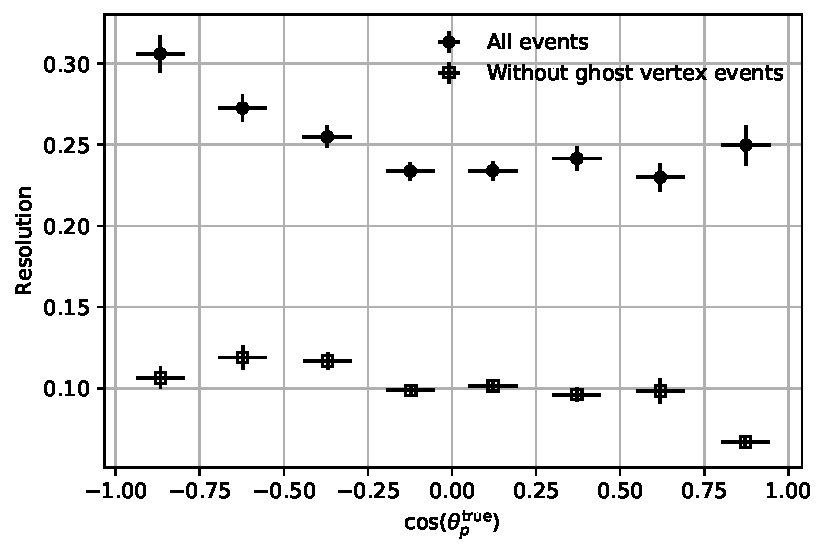
\includegraphics[width=\textwidth]{graphics/05-angular_distributions/MCRECO_p_theta_resolution_nocross.pdf}
		\caption{}
		\label{fig:4:theta_resolution_nocross}
	\end{subfigure}
	\begin{subfigure}{.45\textwidth}
		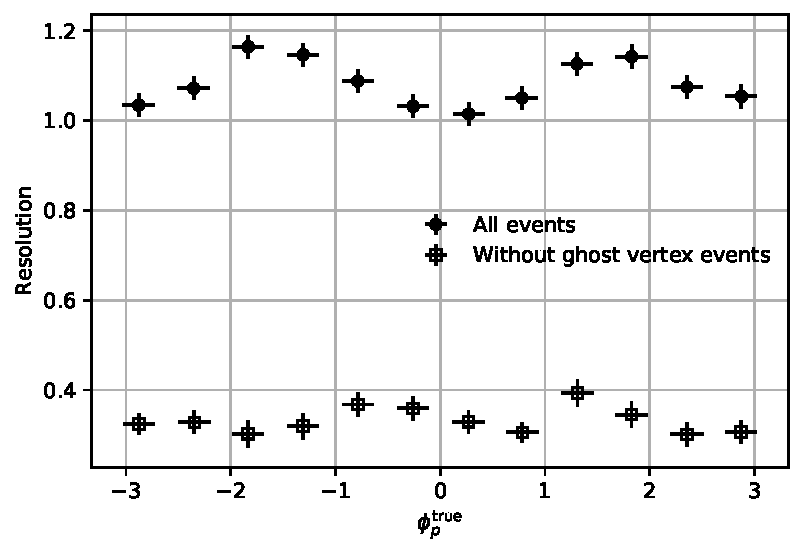
\includegraphics[width=\textwidth]{graphics/05-angular_distributions/MCRECO_p_phi_resolution_nocross.pdf}
		\caption{}
		\label{fig:5:phi_resolution_nocross}
	\end{subfigure}
	\caption{Angular resolutions on $\cos\theta_p$ \textit{(a)} and $\phi_p$ \textit{(b)} as a function of the respective true values. Resolutions are computed on simulated \demonstratorshort events after all selection steps, including (\textit{filled circles}) and removing (\textit{empty squares}) \lambdadecay ghost vertex events.}
	\label{fig:4:resolution_nocross}
\end{figure}
